%%%
% Plantilla de Memoria
% Modificación de una plantilla de Latex de Nicolas Diaz para adaptarla 
% al castellano y a las necesidades de escribir informática y matemáticas.
%
% Editada por: Mario Román
%
% License:
% CC BY-NC-SA 3.0 (http://creativecommons.org/licenses/by-nc-sa/3.0/)
%%%

%%%%%%%%%%%%%%%%%%%%%%%%%%%%%%%%%%%%%%%%%
% Thin Sectioned Essay
% LaTeX Template
% Version 1.0 (3/8/13)
%
% This template has been downloaded from:
% http://www.LaTeXTemplates.com
%
% Original Author:
% Nicolas Diaz (nsdiaz@uc.cl) with extensive modifications by:
% Vel (vel@latextemplates.com)
%
% License:
% CC BY-NC-SA 3.0 (http://creativecommons.org/licenses/by-nc-sa/3.0/)
%
%%%%%%%%%%%%%%%%%%%%%%%%%%%%%%%%%%%%%%%%%

%----------------------------------------------------------------------------------------
%	PAQUETES Y CONFIGURACIÓN DEL DOCUMENTO
%----------------------------------------------------------------------------------------

%%% Configuración del papel.
% microtype: Tipografía.
% mathpazo: Usa la fuente Palatino.
\documentclass[a4paper, 11pt]{article}
\usepackage[protrusion=true,expansion=true]{microtype}
\usepackage{mathpazo}

% Indentación de párrafos para Palatino
\setlength{\parindent}{0pt}
  \parskip=8pt
\linespread{1.05} % Change line spacing here, Palatino benefits from a slight increase by default


%%% Castellano.
% noquoting: Permite uso de comillas no españolas.
% lcroman: Permite la enumeración con numerales romanos en minúscula.
% fontenc: Usa la fuente completa para que pueda copiarse correctamente del pdf.
\usepackage[spanish,es-noquoting,es-lcroman]{babel}
\usepackage[utf8]{inputenc}
\usepackage[T1]{fontenc}
\selectlanguage{spanish}


%%% Gráficos
\usepackage{graphicx} % Required for including pictures
\usepackage{wrapfig} % Allows in-line images
\usepackage[usenames,dvipsnames]{color} % Coloring code

%%% Árboles
\usepackage{tikz}
\usetikzlibrary{automata,arrows}

%%% Matemáticas
\usepackage{amsmath}

%%% Código
\usepackage{listings}

%%% Bibliografía
\makeatletter
\renewcommand\@biblabel[1]{\textbf{#1.}} % Change the square brackets for each bibliography item from '[1]' to '1.'
\renewcommand{\@listI}{\itemsep=0pt} % Reduce the space between items in the itemize and enumerate environments and the bibliography



%----------------------------------------------------------------------------------------
%	TÍTULO
%----------------------------------------------------------------------------------------
% Configuraciones para el título.
% El título no debe editarse aquí.
\renewcommand{\maketitle}{
  \begin{flushright} % Right align
  
  {\LARGE\@title} % Increase the font size of the title
  
  \vspace{50pt} % Some vertical space between the title and author name
  
  {\large\@author} % Author name
  \\\@date % Date
  \vspace{40pt} % Some vertical space between the author block and abstract
  \end{flushright}
}

%% Título
\title{\textbf{Estrella de Steiner en grafos}\\ % Title
Prueba de la NP-completitud} % Subtitle

\author{\textsc{Sofía Almeida Bruno,\\Pablo Álvarez Cabrera} % Author
\\{\textit{Universidad de Granada}}} % Institution

\date{\today} % Date



%----------------------------------------------------------------------------------------
%	DOCUMENTO
%----------------------------------------------------------------------------------------

\begin{document}

\maketitle % Print the title section

%% Resumen (Descomentar para usarlo)
%\renewcommand{\abstractname}{Resumen} % Uncomment to change the name of the abstract to something else
%\begin{abstract}
% Resumen aquí
%\end{abstract}

%% Palabras clave
%\hspace*{3,6mm}\textit{Keywords:} lorem , ipsum , dolor , sit amet , lectus % Keywords
%\vspace{30pt} % Some vertical space between the abstract and first section

%%% Inicio del documento
\section*{Descripción del problema}
El problema de la estrella de Steiner en grafos, al que nos referiremos como ES, se define de la siguiente forma:

Dado un grafo $G=(V,E)$, un subconjunto $R\subseteq V$ y un entero positivo $K \leq V - 1$, ¿existe un subárbol de $G$ que contiene todos los vértices de $R$ y que no contiene más de $K$ arcos?

\section*{NP-completitud}
En primer lugar veremos que está en NP. Después, definiremos una reducción del problema 3-SET al ES para probar que es NP-completo.

\subsection*{ES está en NP}
El algoritmo sería el siguiente:
\begin{itemize}
\item Seleccionar de forma no determinista un subgrafo, esto es, elegir un subconjunto de nodos y otro de aristas.
\item Comprobar que el subgrafo es un árbol. Esto se puede hacer viendo que no contiene ciclos y que es conexo, lo cual se puede hacer en tiempo polinómico.
\item Verificar que contiene a los nodos de $R$.
\item Ver que el subgrafo no contiene más de $K$ arcos.
\end{itemize}

Si existe una estrella de Steiner en el grafo, el algoritmo anterior devuelve ``SÍ'' para un cierto subgrafo. En caso de no existir, el algoritmo devuelve siempre ``NO''.

\subsection*{Reducción 3-SET $\propto$ ES}
Para la reducción vamos a considerar el problema del cubrimiento por conjuntos de tamaño tres (3-SET).

Una instancia de este problema vendrá dada por:
\begin{itemize}
\item Un conjunto finito $X = \{x_1, \dots, x_{3q}\}$.
\item Un subconjunto $C = \{C_1,\dots,C_n\}$ de subconjuntos de $X$ de 3 elementos.
\end{itemize}

La reducción se hará de la siguiente forma:

Queremos construir una entrada $(G=(V,E),R,K)$ para el problema ES a partir de una entrada $(X,C)$ para el problema 3-SET.

\begin{itemize}
\item En el conjunto de vértices habrá un vértice por cada elemento de $X$, otro por cada elemento de $C$ y un vértice al que llamaremos $v$. $$V= \{x_1,\dots,x_{3q}\} \cup \{c_1,\dots, c_n\} \cup \{v\}$$
\item Habrá una arista uniendo $v$ con cada uno de los $c_i$ y otra uniendo cada $c_i$ con los elementos que contiene. $$E = \{vc_1, \dots, vc_n\} \cup (\bigcup_{x_j \in c_i}\{c_ix_j\})$$
\item Consideremos $R = \{v, x_1, \dots, x_{3q}\}$.
\item Por último, $K = 4q$.
\end{itemize}

Veamos que si 3-SET tiene solución positiva, entonces ES también la tiene.

Sea $C'$ un cubrimiento por conjuntos de $X$. Como $|X| = 3q$, $C'$ tendrá $3q/3 = q$ subconjuntos. Supongamos que estos son $c_1,\dots, c_q$. Consideramos el subgrafo dado por $(V,E)$, donde $V=\{v,c_1,\dots,c_q,x_1,\dots,x_{3q}\}$ y $E=\{vc_1,\dots,vc_q\}\cup(\bigcup_{x_j \in c_i}\{c_ix_j\})$ con $i=1,\dots,q$. Esta es la estrella de Steiner que resuelve el problema, ya que se trata de un árbol que contiene a los nodos de $R$ y el número de aristas es $q+3q = 4q = k$.

Finalizaremos viendo que si ES tiene una solución positiva, entonces 3-SET también la tiene.

Supongamos que existe un grafo de Steiner $G$ con al menos $4q$ lados. Como $G$ es un árbol no puede tener más de $4q+1$ vértices. $G$ contiene a $v$ y $x_1,\dots,x_{3q}$, luego no puede incluir más de $q$ vértices $c_i$. Ahora observamos que para conectar con todos los nodos $x_i$ debe haber al menos $4q+1$ vértices, luego $G$ contiene exactamente $4q$ aristas y $q$ nodos $c_i$ ($c_1,\dots,c_q$). La solución al problema 3-SET vendrá dada por los subconjuntos $C_1,\dots,C_q$ asociados a los vértices $c_1,\dots,c_q$.

\subsubsection*{Espacio logarítmico}

Veamos que esta reducción se puede hacer en espacio logarítmico. Supongamos que la entrada tiene el siguiente formato: $$x_1 \dots x_{3q} \# c_{11} c_{12} c_{13} \dots c_{n1} c_{n2} c_{n3}$$ La salida estará formada por el listado de vértices seguido por el listado de aristas, el valor de $R$ y el valor de $K$ separados por $\#$.

Para los vértices, basta con escribir $v$, ir copiando en la salida los elementos de la entrada hasta llegar a $\#$ y a partir de ahí añadir $c_i$ por cada tres elementos. Por tanto, será necesario un contador $i=1,\dots,n$ y otro $j=1,2,3$  que se pueden almacenar en espacio logarítmico (en binario).

Para las aristas, volvemos hasta el símbolo $\#$ en la entrada y vamos avanzando escribiendo las aristas $vc_{i},\ c_ic_{ij}, \quad i=1,\dots,n \quad j=1,\dots,3$ (usamos los mismos contadores).

Para $R$, volvemos hacia el comienzo de la entrada y añadimos $v$ seguido de $x_1 \dots x_3q$. Guardamos en otro contador el valor $3q$ (también es espacio logarítmico).

Por último, escribimos $K = 4q$ (multiplicar y dividir en binario se puede hacer en espacio logarítmico).

El funcionamiento del algoritmo queda ilustrado en el código que hemos implementado en Python:

% Código
\lstinputlisting[language=Python, firstline=3]{reduction.py}

\subsection*{Ejemplo}
Veamos cómo funciona la reducción en un caso concreto.

Partimos del problema 3-SET dado por$X=\{x_1,\dots,x_q\}$ y $C=\{C_1,\dots,C_5\}$, donde $C_1=\{x_2, x_5, x_7\}$, $C_2=\{x_1,x_3,x_4\}$, $C_3=\{x_6,x_8,x_9\}$, $C_4=\{x_2,x_3,x_6\}$, $C_5=\{x_7,x_8,x_9\}\}$. Este problema admite como solución $C'=\{C_1,C_2,C_3\}$.

La entrada de la reducción serían los conjuntos $X, C$ y la salida, el grafo mostrado a continuación, $R=\{v,x_1,\dots,x_9\}$, $K=12$.\\

\tikzstyle{selected}=[draw=green,fill=green!30]
\begin{tikzpicture}[>=stealth',shorten >=1pt,auto,node distance=1.8 cm, scale = 1, transform shape, initial text=]

  \tikzstyle{state}=[circle,thick,draw=blue!150,fill=blue!20,minimum size=6mm]


  \node[state] 	[selected] (v)  	{$v$};
 
  \node[state]  [selected] (c3) [below of=v]    {$c_3$};
  \node[state]  [selected] (c2) [left of=c3]    {$c_2$};
  \node[state]  [selected] (c1) [left of=c2]    {$c_1$};
  \node[state]  (c4) [right of=c3] 	 {$c_4$};
  \node[state]  (c5) [right of=c4]       {$c_5$};

  
  \node[state] [selected] (x5) [below of=c3]       {$x_5$};
  \node[state] [selected] (x4) [left  of=x5]       {$x_4$};
  \node[state] [selected] (x3) [left  of=x4]       {$x_3$};
  \node[state] [selected] (x2) [left of=x3]        {$x_2$};
  \node[state] [selected] (x1) [left of=x2]        {$x_1$};
  \node[state] [selected] (x6) [right of=x5]       {$x_6$};
  \node[state] [selected] (x7) [right of=x6]       {$x_7$};
  \node[state] [selected] (x8) [right of=x7]       {$x_8$};
  \node[state] [selected] (x9) [right of=x8]       {$x_9$};

  \path[--]
  (v) edge (c1)
  (v) edge (c2)
  (v) edge (c3)
  (v) edge (c4)
  (v) edge (c5)
  (c1) edge (x2)
  (c1) edge (x5)
  (c1) edge (x7)
  (c2) edge (x1)
  (c2) edge (x3)
  (c2) edge (x4)
  (c3) edge (x6)
  (c3) edge (x8)
  (c3) edge (x9)
  (c4) edge (x2)
  (c4) edge (x3)
  (c4) edge (x6)
  (c5) edge (x7)
  (c5) edge (x8)
  (c5) edge (x9)

\end{tikzpicture}


Una solución a este problema es el subárbol formado por los nodos coloreados en verde y las aristas que los unen.

% Imagen ejecución
Ejecutamos nuestro programa pasándole como entrada este mismo ejemplo y obtenemos:

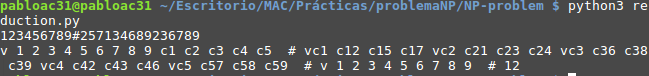
\includegraphics[width=13cm]{imagen}

\end{document}
